\documentclass[a4paper,english]{scrreprt}

% Uncomment to optimize for double-sided printing.
% \KOMAoptions{twoside}

% Set binding correction manually, if known.
% \KOMAoptions{BCOR=2cm}

% Localization options
\usepackage[english]{babel}
\usepackage[T1]{fontenc}
\usepackage[utf8]{inputenc}

% Enhanced verbatim sections. We're mainly interested in
% \verbatiminput though.
\usepackage{verbatim}

% PDF-compatible landscape mode.
% Makes PDF viewers show the page rotated by 90°.
\usepackage{pdflscape}

% Advanced tables
\usepackage{tabu}
\usepackage{longtable}
\usepackage{dcolumn}
\newcolumntype{d}[1]{D{.}{\cdot}{#1} }

% Fancy tablerules
\usepackage{booktabs}

% Graphics
\usepackage{graphicx}

% Current time
\usepackage[useregional=numeric]{datetime2}

% Float barriers.
% Automatically add a FloatBarrier to each \section
\usepackage[section]{placeins}

% Custom header and footer
\usepackage{fancyhdr}

\usepackage{geometry}
\usepackage{layout}

% Math tools
\usepackage{mathtools}
% Math symbols
\usepackage{amsmath,amsfonts,amssymb}
\usepackage{amsthm}

% SI units
\usepackage{siunitx}
\DeclareSIUnit\Molar{\textsc{m}}
\DeclareSIUnit\mole{mol}
\DeclareSIUnit\rpm{rpm}
\DeclareSIUnit\cfu{cfu}

% Chemistry
\usepackage{mhchem}

% Subfigures & captions
\usepackage{subcaption}
\usepackage{wrapfig}

\DeclarePairedDelimiter\abs{\lvert}{\rvert}

\pagestyle{plain}
% \fancyhf{}
% \lhead{}
% \lfoot{}
% \rfoot{}
% 
% Source code & highlighting
\usepackage{listings}

% Convenience commands
\newcommand{\mailsubject}{2027 - Lab course biochemistry 1}
\newcommand{\maillink}[1]{\href{mailto:#1?subject=\mailsubject}
                               {#1}}

% Should use this command wherever the print date is mentioned.
\newcommand{\printdate}{\today}

\subject{2027 - Lab course biochemistry 1}

\title{4 - Enzymkinetik mit Katalase}

\author{Michael Senn \maillink{michael.senn@students.unibe.ch} - 16-126-880 - Gruppe 14}

\date{\printdate}

% Needs to be the last command in the preamble, for one reason or
% another. 
\usepackage{hyperref}


\begin{document}
\maketitle

\chapter{Introduction}

Enzymes are a class of proteins which accelerate certain reactions by several
orders of magnitude. They are often specific to one kind of reaction, which
they catalyze by eg increasing the stability of intermediary products, base and
acid reactions, or influencing the spatial orientiation of molecules involved
in the reaction.

Enzyme activity is often influenced by various environmental factors, such as
temperature, the concentration of enzyme and substrate and the pH value.

Catalase is one such enzyme which catalyzes the decay of \ce{H2O2} to \ce{H2O}
and \ce{O2}. This prevents the buildup of toxic \ce{H2O2} in cells, which is
the result of the reduction of \ce{O2-} radicals.

In this experiment we aim to characterize the enzymatic activity of catalse
under varying environmental factors.

\chapter{Methods}

To characterize activity of catalase under various constraints, the cytosol -
containing large concentrations of catalase - of potatoes was isolated. A small
amount of this solution was applied onto a small filter paper, which was then
submerged into a solution containing \ce{H2O2}.

The decomposition of \ce{H2O2} by the catalase lead to the formation of oxygen
bubbles, some of which attached to the filter paper. Once enough oxygen was
attached, the filter paper rose to the surface.

The time between the submerging and the resurfacing of the filter paper was
measured, and taken as an indication of the activity of catalse under the given
circumstances.

\chapter{Results}

\section{Calculating ideal concentration of enzyme}

\subsection{Experiment}

To start with, the ideal enzymatic concentration was determined. The aim was to
have a concentration where the filter resurfaces slow enough that time can be
measured accurately, and fast enough that difusion of the enzyme does not
influence results significantly.

To achieve this, the dilutions shown in table \ref{tbl:enzyme_dilutions} were
prepared, applied to a filter, and each submerged in \SI{60}{\ml}
\SI{1}{\percent} \ce{H2O2}.

\begin{table}
	\centering
	\begin{tabu}{lllll}
		\toprule
		& E1 & E2 & E3 & E4 \\
		\midrule
		Cell extract & \SI{10}{\ml} & \SI{10}{\ml} & \SI{5}{\ml} & \SI{0}{\ml} \\
		Cold water & \SI{0}{\ml} & \SI{10}{\ml} & \SI{15}{\ml} & \SI{20}{\ml} \\
		Concentration (given) & \SI{100}{U \per \ml}& \SI{50}{U \per \ml} & \SI{25}{U \per \ml} & \SI{0}{U \per \ml} \\
		\bottomrule
	\end{tabu}
	\caption{Enzyme dilutions for determining ideal concentration}
	\label{tbl:enzyme_dilutions}
\end{table}

\subsection{Raw data}

Each measurement was done thrice, with results shown in table \ref{tbl:enzyme_dilutions_time}.

\begin{table}
	\centering
	\begin{tabu}{lllll}
		\toprule
		& E1 & E2 & E3 & E4 \\
		\midrule
		Measurement 1 & \SI{14}{\s} & \SI{14}{\s} & \SI{20}{\s} & - \\
		Measurement 2 & \SI{12}{\s} & \SI{17}{\s} & \SI{18}{\s} & - \\
		Measurement 3 & \SI{15}{\s} & \SI{13}{\s} & \SI{22}{\s} & - \\
		\bottomrule
	\end{tabu}
	\caption{Resurfacing time under various enzyme concentrations}
	\label{tbl:enzyme_dilutions_time}
\end{table}

\subsection{Reaction speed as factor of enzyme concentration}

The surfacing velocity was calculated as the reciprocal of the surfacing time,
and the average and standard deviation of each calculated. These were graphed
against the provided enzyme concentrations of the four samples, and a linear
regression with a forced intercept through the origin calculated, as shown in
figure \ref{fig:enzyme_optimal_concentration}.

\begin{figure}
	\centering
	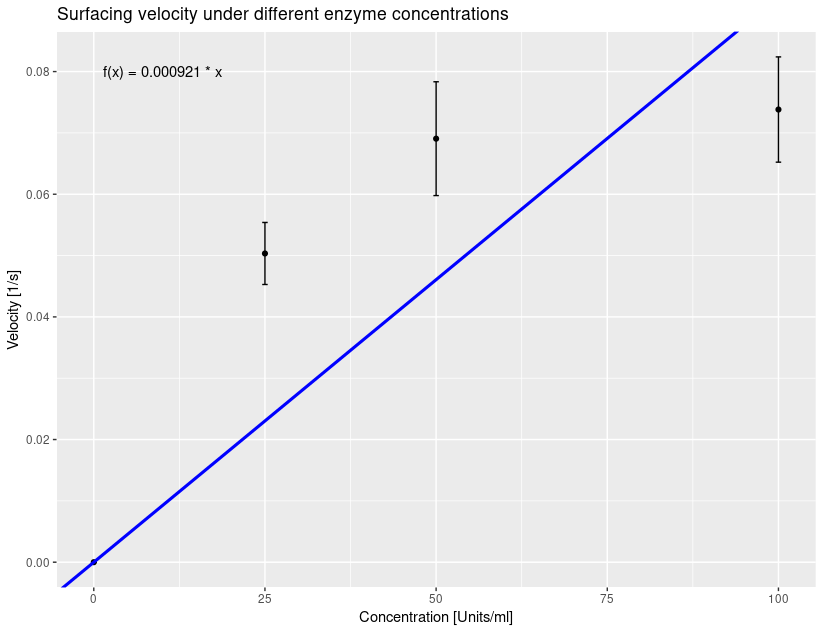
\includegraphics[width=0.9\textwidth]{img/optimal_concentration.png}
	\caption{Resurfacing velocity under various enzyme concentrations}
	\label{fig:enzyme_optimal_concentration}
\end{figure}

It is clearly visible that, as enzyme concentration increases, so does the the
resurfacing velocity. This matches the expectation that presence of more enzyme
will increase the number of reactions catalyzed per second. There seems to be a
saturation effect, where reaction velocity does not increase a lot beyond an
enzyme concentration of \SI{100}{U \per \ml}. Additional measurements at higher
concentrations would be required to verify this, however.

\subsection{Determining ideal enzyme concentration}

Using the equation of the calculated regression we were able to calculate the
concentration where the resurfacing time will be at \SI{20}{\s} as:

\[
	0.000921 \cdot x = \frac{1}{20} \Rightarrow x \approx 54.3
\]

As this was close enough to the \SI{50}{U \per \ml} concentration of one of our
existing dilutions, we continued using this one for future experiments.

\section{Determining $K_m$}

\subsection{Experiment}

In the next experiment we measured resurfacing time in solutions with different
concentrations of the substrate, as shown in table
\ref{tbl:substrate_concentration}.

\begin{table}
	\centering
	\begin{tabu}{llllllll}
		\toprule
		& S11 & S12 & S13 & S14 & S15 & S16 & S17 \\
		\midrule
		\ce{H2O} & \SI{40}{\ml} & \SI{50}{\ml} & \SI{58}{\ml} & \SI{58.4}{\ml} & \SI{59}{\ml} & \SI{59.6}{\ml} & \SI{60}{\ml} \\
		\ce{H2O2} \SI{30}{\percent} & \SI{20}{\ml} & \SI{10}{\ml} & \SI{2}{\ml} & \SI{1.6}{\ml} & \SI{1}{\ml} & \SI{0.4}{\ml} & \SI{0}{\ml} \\
		Concentration \ce{H2O2} & \SI{10}{\percent} & \SI{5}{\percent} & \SI{1}{\percent} & \SI{0.8}{\percent} & \SI{0.5}{\percent} & \SI{0.2}{\percent} & \SI{0}{\percent} \\
		\bottomrule
	\end{tabu}
	\caption{Different substrate concentrations for determining $K_m$}
	\label{tbl:substrate_concentration}
\end{table}

\subsection{Raw data}

Each measurement was done thrice, with results shown in table
\ref{tbl:substrate_concentrations_time}.

\begin{table}
	\centering
	\begin{tabu}{llllllll}
		\toprule
		& S11 & S12 & S13 & S14 & S15 & S16 & S17 \\
		\midrule
		Measurement 1 & \SI{2}{\s} & \SI{7}{\s} & \SI{19}{\s} & \SI{29}{\s} & \SI{18}{\s} & \SI{47}{\s} & - \\ 
		Measurement 2 & \SI{3}{\s} & \SI{7}{\s} & \SI{15}{\s} & \SI{26}{\s} & \SI{25}{\s} & \SI{50}{\s} & - \\ 
		Measurement 3 & \SI{3}{\s} & \SI{6}{\s} & \SI{17}{\s} & \SI{32}{\s} & \SI{23}{\s} & \SI{42}{\s} & - \\ 
		\bottomrule
	\end{tabu}
	\caption{Resurfacing time under various substrate concentrations}
	\label{tbl:substrate_concentrations_time}
\end{table}

\subsection{Reaction speed as factor of enzyme concentration}

As before the average surface velocity was calculated and graphed against the
concentration of the substrate, shown in figure
\ref{fig:substrate_concentration}.

\begin{figure}
	\centering
	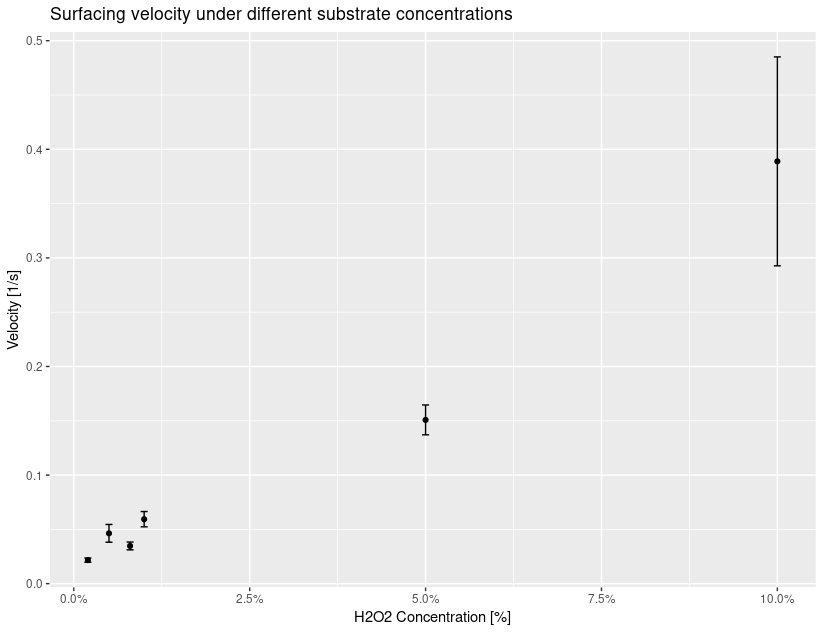
\includegraphics[width=0.9\textwidth]{img/substrate_concentration.png}
	\caption{Resurfacing velocity under various substrate concentrations}
	\label{fig:substrate_concentration}
\end{figure}

As expected, increasing the substrate concentration leads to an increase in
reaction speed. This implies that the reaction is also limited by the
concentration of substrate, due to the requirement that enzyme and substrate
meet for the reaction to proceed.

There is, however, no saturation visible. This prevents reliably estimating
$K_m$, as it is defined to be the substrate concentration where the enzymatic
reaction is at half the maximum speed. 

It is possible that substrate concentration would have had to be increased even
higher in order to enter an area of substrate saturation, where the increase in
reaction speed would have slowed down. To prevent inaccuracies in time
measurement, the enzyme concentration would also have had to be reduced, as
even with \SI{10}{\percent} \ce{H2O2} resurfacing time was around
\SIrange{2}{3}{\s}.

However, a concentration per volume of \SI{10}{\percent}, with \ce{H2O2}'s
density of \SI{1.11}{\g \per \cm^3} is equal to \SI{111}{\g \per \l}, which
with its molecular weight of \SI{34}{\g \per \mol} implies an already high
molarity of \SI{3.2}{\Molar}.

\subsection{Calculating $K_m$}

\begin{figure}
	\centering
	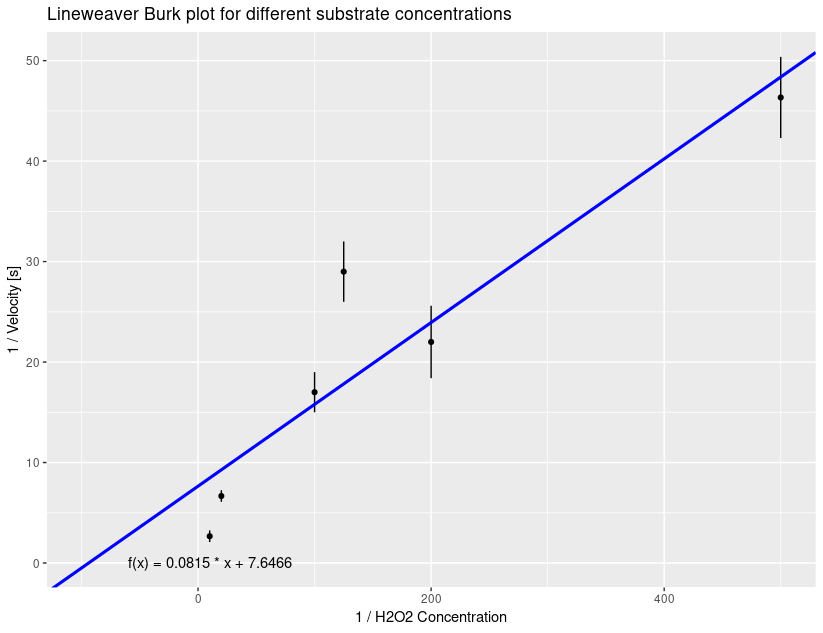
\includegraphics[width=0.9\textwidth]{img/substrate_concentration_lburk.png}
	\caption{Lineweaver Burk plot for different substrate concentrations}
	\label{fig:substrate_concentration_lburk}
\end{figure}

With that in mind, $K_m$ was estimated with a double reciprocal Lineweaver-Burk
plot coupled with a linear regression seen in figure
\ref{fig:substrate_concentration_lburk}.

From its expression, the X intercept can be calculated as
\begin{align*}
	0 & = 0.0815 * x + 7.6466 \\
	x & = \frac{-7.6466}{0.0815} \\
	x & \approx -93.8
\end{align*}

As the X axis intercept is equal to $-\frac{1}{K_m}$, it follows that $K_m
\approx \SI{0.01}{\percent}$.

\section{pH dependance of reaction speed}

\subsection{Experiment}

Next, the influence of pH on reaction velocity was investigated. For that, four
solutions of \SI{1}{\percent} \ce{H2O2} were prepared, and their pH set  with a
\ce{K2HPO4} / \ce{KH2PO4} buffer.

\begin{description}
	\item[S21] pH 4
	\item[S22] pH 6
	\item[S23] pH 8
	\item[S24] pH 9.4
\end{description}

\subsection{Raw data}

Each measurement was done twice, with results shown in table
\ref{tbl:ph_time}.

\begin{table}
	\centering
	\begin{tabu}{lllll}
		\toprule
		& S21 & S22 & S23 & S24 \\
		\midrule
		Measurement 1 & \SI{59}{\s} & \SI{27}{\s} & \SI{18}{\s} & \SI{18}{\s} \\ 
		Measurement 2 & \SI{66}{\s} & \SI{26}{\s} & \SI{16}{\s} & \SI{17}{\s} \\ 
		\bottomrule
	\end{tabu}
	\caption{Resurfacing time under various pH levels}
	\label{tbl:ph_time}
\end{table}

\subsection{Reaction speed as factor of pH value}

Once more, average surface velocity was calculated and graphed, shown in figure
\ref{fig:ph}.

\begin{figure}
	\centering
	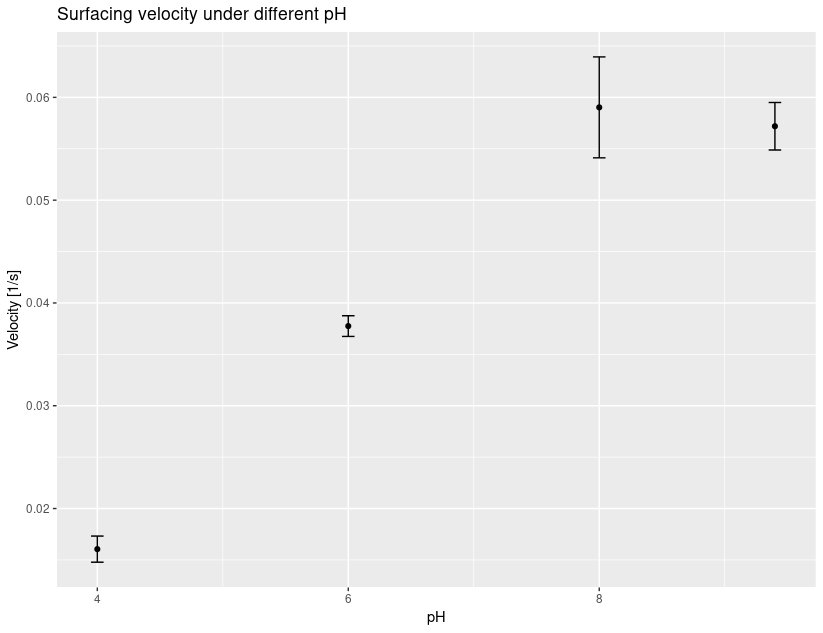
\includegraphics[width=0.9\textwidth]{img/ph.png}
	\caption{Resurfacing velocity under various pH levels}
	\label{fig:ph}
\end{figure}

As visible in the graph, an acidic pH heavily lowers the reaction speed. The
highest observed speed was achieved at a pH of 8, which matches the expectation
of the enzyme being most efficient near neutral pH levels found within many
organism's cells.

Of interest is that a basic pH at 9.4 did not lower reaction speed
significantly, indicating that the enzyme is not extremely sensitive to
slightly basic pH values.

\section{Inhibition of enzyme via hydroxylamine}

\subsection{Experiment}

Lastly, the effect of inhibition with hydroxylamine was looked at, to determine
if inhibition is competitive - in which case inhibitor and substrate occupy the
same binding site - or non-competitive in which case the inhibitor causes eg a
change in conformation which deactivates the enzyme.

Three measurement series were prepared, with different concentrations of
\ce{H2O2} according to table \ref{tbl:substrate_concentration}, containing
hydroxylamine concentrations of \SI{2.5E-6}{\percent}, \SI{5E-6}{\percent} and
\SI{2E-5}{\percent} respectively.


\subsection{Raw data}

Each measurement was done twice, with results shown in table
\ref{tbl:inhibition_time}.

\begin{table}
	\centering
	\begin{tabu}{llllllll}
		\toprule
		& S11 & S12 & S13 & S14 & S15 & S16 & S17 \\
		\midrule
		\multicolumn{8}{c}{\SI{2.5E-6}{\percent}} \\
		\midrule
		Measurement 1 & \SI{4}{\s} & \SI{11}{\s} & \SI{22}{\s} & \SI{46}{\s} & \SI{43}{\s} & \SI{73}{\s} & - \\ 
		Measurement 2 & \SI{6}{\s} & \SI{8}{\s}  & \SI{23}{\s} & \SI{46}{\s} & \SI{39}{\s} & \SI{70}{\s} & - \\ 
		Measurement 3 & \SI{6}{\s} & \SI{8}{\s}  & \SI{23}{\s} & \SI{43}{\s} & \SI{35}{\s} & \SI{69}{\s} & - \\ 
		\midrule
		\multicolumn{8}{c}{\SI{5E-6}{\percent}} \\
		\midrule
		Measurement 1 & \SI{6}{\s} & \SI{11}{\s} & \SI{26}{\s} & \SI{68}{\s} & \SI{74}{\s} & \SI{165}{\s} & - \\ 
		Measurement 2 & \SI{6}{\s} & \SI{10}{\s} & \SI{34}{\s} & \SI{63}{\s} & \SI{95}{\s} & \SI{120}{\s} & - \\ 
		Measurement 3 & \SI{7}{\s} & \SI{10}{\s} & \SI{32}{\s} & \SI{67}{\s} & \SI{67}{\s} & \SI{140}{\s} & - \\ 
		\midrule
		\multicolumn{8}{c}{\SI{2E-5}{\percent}} \\
		\midrule
		Measurement 1 & \SI{25}{\s} & \SI{35}{\s} & \SI{91}{\s} & \SI{120}{\s} & \SI{130}{\s} & \SI{385}{\s} & - \\ 
		Measurement 2 & \SI{21}{\s} & \SI{37}{\s} & \SI{96}{\s} & \SI{146}{\s} & \SI{160}{\s} & \SI{745}{\s} & - \\ 
		Measurement 3 & \SI{20}{\s} & \SI{38}{\s} & \SI{97}{\s} & \SI{172}{\s} & \SI{157}{\s} & \SI{730}{\s} & - \\ 
		\bottomrule
	\end{tabu}
	\caption{Resurfacing time under various substrate concentrations and inhibition levels}
	\label{tbl:inhibition_time}
\end{table}


\subsection{Reaktion speed as factor of enzyme inhibition}

The calculatd velocities per substrate and hydroxylamine concentrations were
graphed, as velocity over concentration shown in figure \ref{fig:inhibition},
as well as the double reciprocal of 1/velocity over 1/concentration shown in
figure \ref{fig:inhibition_lburk}.

\begin{figure}
	\centering
	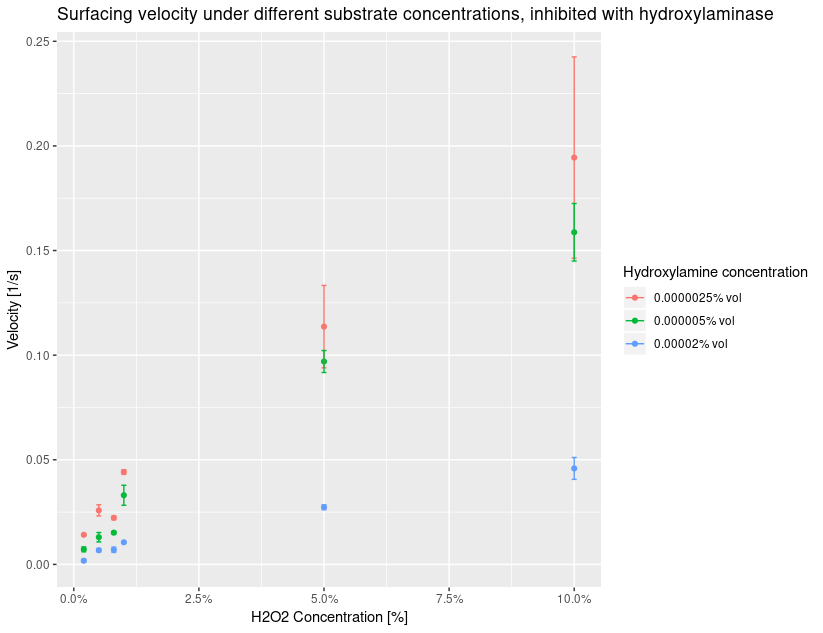
\includegraphics[width=0.9\textwidth]{img/inhibition.png}
	\caption{Resurfacing velocity under various substrate and inhibitor concentrations}
	\label{fig:inhibition}
\end{figure}

\begin{figure}
	\centering
	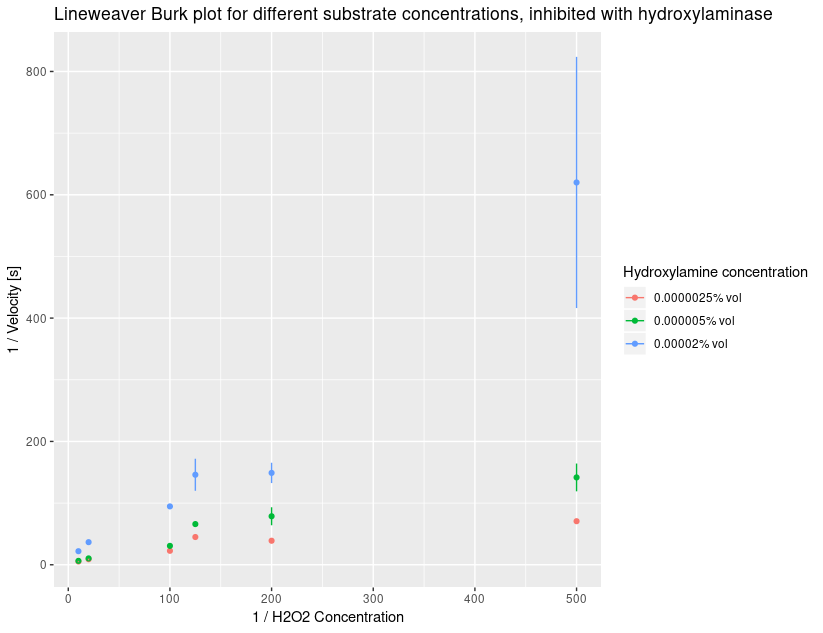
\includegraphics[width=0.9\textwidth]{img/inhibition_lburk.png}
	\caption{Lineweaver Burk plot for different substrate and inhibitor concentrations}
	\label{fig:inhibition_lburk}
\end{figure}

In the Lineweaver Burk plot in figure \ref{fig:inhibition_lburk} it is evident
that, as concentration of Hydroxylaminase goes up, the slope increases. This
implies that inhibition is competitive, with Hydroxylaminase and \ce{H2O2}
competing for the same binding site within catalase.

\chapter{Conclusion}

In conclusion, we have shown that increasing both substrate as well as enzyme
concentration increase reaction speed. Furthermore, the enzyme is most active
between a pH of 8 and 9.

We were unable to reliably determine $K_m$ as no substrate saturation could be
observed. This was likely due to a mistake in the experiment's execution,
rather than not having reached the point where saturation should occur.

We did however show that Hydroxylaminase seems to be a competitive inhibitor of
catalase.

\bibliographystyle{vancouver}
\bibliography{references}

\end{document}
